\begin{pastexam}[label={px:ust-110-ee-ds-10}]{臺聯大電機類 110 學年度 第 10 題}
（問答）

(10\%) The shell sort algorithm is an improved version of the straight insertion sort. In the shell sort,
a list of $N$ elements is divided into $K$ segments, where $K$ is known as the increment. For example, in
Figure 3, $K$ is 3. The first, fourth, seventh, and tenth elements make up segment 1. For each pass, the data
in each segment are sorted in \textbf{Insertion Sort}. Thus, after insertion sort, there are three different
ordered lists. After each pass through the data, the increment is divided by two ($K$/2) until, in the final
pass, it is 1. Please prove (explain) the time complexity of Shell sort is close to O($N$ log $N$).

\begin{center}
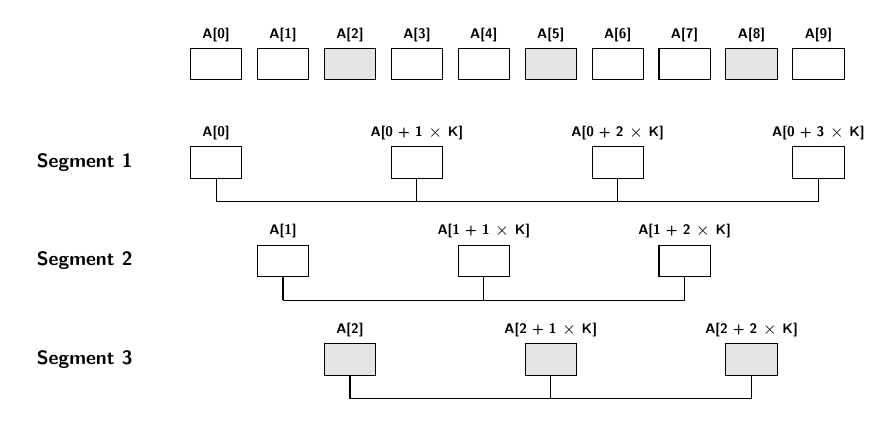
\begin{tikzpicture}[l/.style={font=\tiny\bfseries\sffamily,inner sep=0pt,anchor=south},b/.style={draw,minimum width=6.5mm,minimum height=4mm,inner sep=0pt}]
\node[b] at (0.00,0) {};\node[l] at (0.00,0.28) {A[0]};
\node[b] at (0.85,0) {};\node[l] at (0.85,0.28) {A[1]};
\node[b,fill=gray!20] at (1.70,0) {};\node[l] at (1.70,0.28) {A[2]};
\node[b] at (2.55,0) {};\node[l] at (2.55,0.28) {A[3]};
\node[b] at (3.40,0) {};\node[l] at (3.40,0.28) {A[4]};
\node[b,fill=gray!20] at (4.25,0) {};\node[l] at (4.25,0.28) {A[5]};
\node[b] at (5.10,0) {};\node[l] at (5.10,0.28) {A[6]};
\node[b] at (5.95,0) {};\node[l] at (5.95,0.28) {A[7]};
\node[b,fill=gray!20] at (6.80,0) {};\node[l] at (6.80,0.28) {A[8]};
\node[b] at (7.65,0) {};\node[l] at (7.65,0.28) {A[9]};
\node[font=\scriptsize\bfseries\sffamily,anchor=west] at (-2.4,-1.25) {Segment 1};
\node[b] at (0.00,-1.25) {};\node[l] at (0.00,-0.97) {A[0]};
\draw (0.00,-1.45)--(0.00,-1.75);
\node[b] at (2.55,-1.25) {};\node[l] at (2.55,-0.97) {A[0 + 1 $\times$ \textit{K}]};
\draw (2.55,-1.45)--(2.55,-1.75);
\node[b] at (5.10,-1.25) {};\node[l] at (5.10,-0.97) {A[0 + 2 $\times$ \textit{K}]};
\draw (5.10,-1.45)--(5.10,-1.75);
\node[b] at (7.65,-1.25) {};\node[l] at (7.65,-0.97) {A[0 + 3 $\times$ \textit{K}]};
\draw (7.65,-1.45)--(7.65,-1.75);
\draw (0.00,-1.75)--(7.65,-1.75);
\node[font=\scriptsize\bfseries\sffamily,anchor=west] at (-2.4,-2.50) {Segment 2};
\node[b] at (0.85,-2.50) {};\node[l] at (0.85,-2.22) {A[1]};
\draw (0.85,-2.70)--(0.85,-3.00);
\node[b] at (3.40,-2.50) {};\node[l] at (3.40,-2.22) {A[1 + 1 $\times$ \textit{K}]};
\draw (3.40,-2.70)--(3.40,-3.00);
\node[b] at (5.95,-2.50) {};\node[l] at (5.95,-2.22) {A[1 + 2 $\times$ \textit{K}]};
\draw (5.95,-2.70)--(5.95,-3.00);
\draw (0.85,-3.00)--(5.95,-3.00);
\node[font=\scriptsize\bfseries\sffamily,anchor=west] at (-2.4,-3.75) {Segment 3};
\node[b,fill=gray!20] at (1.70,-3.75) {};\node[l] at (1.70,-3.47) {A[2]};
\draw (1.70,-3.95)--(1.70,-4.25);
\node[b,fill=gray!20] at (4.25,-3.75) {};\node[l] at (4.25,-3.47) {A[2 + 1 $\times$ \textit{K}]};
\draw (4.25,-3.95)--(4.25,-4.25);
\node[b,fill=gray!20] at (6.80,-3.75) {};\node[l] at (6.80,-3.47) {A[2 + 2 $\times$ \textit{K}]};
\draw (6.80,-3.95)--(6.80,-4.25);
\draw (1.70,-4.25)--(6.80,-4.25);
\end{tikzpicture}\\[2pt] Figure 3. Segments in Shell sort.\end{center}
\end{pastexam}

\begin{pastsoln}
先說結論：題目要的是下面「為什麼接近 $O(N \log N)$」的直觀說明；但嚴格來說，題目描述的這種增量（每次
除以 $2$，Shell 原本的序列）\textbf{最壞情況是 $\Theta(N^2)$}，不是 $O(N \log N)$，平均情況也沒有
$O(N \log N)$ 的證明。 作答時兩件事都寫出來比較完整。 記號照資結書第~14.3~節。

\textbf{直觀說明（題目要的）。}
\begin{enumerate}
\item \textbf{趟數}：增量從 $K \approx N/2$ 開始每次減半，到 $1$ 為止，共 $\lfloor \lg N \rfloor$ 趟左右。
\item \textbf{第一趟}：增量 $K$ 時有 $K$ 段，每段約 $N/K$ 個。 增量很大時每段很短，插入排序的成本是
每段 $O((N/K)^2)$，合計 $K \cdot (N/K)^2 = N^2/K$；$K \approx N/2$ 時只有 $O(N)$。
\item \textbf{後面幾趟}：增量變小、每段變長，但前面幾趟已經把每個數大致搬到正確的區域，陣列「差不多排好
了」。 插入排序的時間是 $\Theta(N + I)$，$I$ 是逆序對個數（資結書第~14.2~節）；如果每一趟每個數只需要往前
挪幾個位置，這一趟就只花 $O(N)$。
\item 合起來：大約 $\lg N$ 趟、每趟大約 $O(N)$，總共大約 $O(N \lg N)$。
\end{enumerate}
直接插入排序是 $\Theta(N^2)$，原因是一個很小的數放在最後面時，必須一格一格挪到前面；Shell 排序先用大的
間隔讓它一次跳 $K$ 格，所以快得多。

\textbf{為什麼只是「接近」：上面第 3 點不保證成立。}
\begin{itemize}
\item \textbf{最壞情況 $\Theta(N^2)$}：$N$ 是 $2$ 的次方時，除了最後的 $1$，每個增量都是偶數，奇數位置和偶數位置
的數在最後一趟之前從不互相比較。 把最小的一半放在奇數位置、最大的一半放在偶數位置（例如 $N = 8$：
$1, 5, 2, 6, 3, 7, 4, 8$），前面每一趟都什麼都沒搬，最後一趟還有 $\frac{N}{2}\left(\frac{N}{2} - 1\right)/2$ 個
逆序對要一個一個挪，$\Theta(N^2)$（資結書第~14.3~節的例子：$N = 4096$ 時最後一趟要挪 $2{,}096{,}128$ 次）。
\item \textbf{亂數輸入}：比較次數除以 $N \lg N$ 不是常數，會隨 $N$ 慢慢變大。 用亂數實測，$N$ 從 $10^3$ 到約
$10^6$，這個比值大約從 $1.5$ 漲到 $5.9$，所以成長得比 $N \lg N$ 快；只是在常見的 $N$ 範圍裡看起來差不多。
\end{itemize}

\textbf{換增量就能改善。} 增量序列決定了複雜度：Hibbard 的 $2^k - 1$ 最壞 $\Theta(N^{3/2})$，Sedgewick 的序列最壞
$O(N^{4/3})$，Pratt 的 $2^p 3^q$ 最壞 $\Theta(N \lg^2 N)$（資結書第~14.3~節的表）。 所以 Shell 排序的時間「介於
$N \lg N$ 和 $N^2$ 之間，看增量而定」才是精確的說法。
\end{pastsoln}
